\newcommand{\urlrref}{http://bmw.byuimath.com/dokuwiki/doku.php?id=rref\_calculator}

\note{next time, should I introduce the words, ``Coordinates of a vector relative to the pivot columns.''?  If I introduced this, then I would have begun a key idea.  Perhaps instead, this should be in the application chapter.  It introduces the ideas needed for talking about all solutions of a differential equation, by talking about the coordinates of a solution relative to the basis of solutions.  I do think this is a good start.}


After completing this chapter, you should be able to:

\begin{enumerate}
\item Explain the difference between linearly independent and linearly dependent. When vectors are linearly dependent, write one of the vectors as a linear combination of the others. 
\item Solve systems of equations by obtain the reduced row echelon form (rref) of a matrix (Gauss-Jordan elimination).
\item Explain how to compute the inverse of a matrix. Then use the inverse to solve various problems such as finding $\vec x$ in $A\vec x = \vec b$ or finding $A$ in $AQ=QD$. 
\item Show how to compute the determinant of a square matrix of any size. Be able to articulate the connection among determinants, linear dependence, and invertibility. 
\item Explain how to see eigenvectors and the sign of eigenvalues in a vector field. Then use this knowledge to show how to obtain eigenvalues and eigenvectors from determinant and row reduction computations. 
\end{enumerate}

%Technology links, especially to RREF.

\newcommand{\ideagau}{Solving Systems of Equations}
\newcommand{\ideaind}{Linear Independence and Dependence}
\newcommand{\ideamul}{Matrix Multiplication and Inverses}
\newcommand{\ideadet}{Applications of Determinants}
\newcommand{\ideaeig}{Seeing Eigenvectors in Vector Fields}



\mysubsection{\ideaind}

The heart of linear algebra has to deal with understanding relationships between vectors.  Vectors give us directions of motion.  They tell us how forces act on objects. We've seen already that vectors provide us with visual solutions to differential equations. One of our goals in this chapter is to become comfortable with working with linear combinations of vectors.  
\marginpar{You may want to review the formal definition of a linear combination. See Definition \ref{def linear combination} on \pageref{def linear combination}.}
Remember that given $n$ vectors  $\vec v_1, \vec v_2,\cdots,\vec v_n$ and $n$ scalars $c_1, c_2, \cdots, c_n$ we say their linear combination is the sum $$c_1\vec v_1+c_2\vec v_2+\cdots+c_n\vec v_n.$$

\begin{problem}\label{sally in corn field with 2 directions}
Sally is trying to find a treasure that's located in a corn field (she's geocaching). 
Her position is currently at $(0,0)$, and she knows that the treasure is located at $(6,8)$ (units are hundreds of yards). 
She can't walk in a straight line to the treasure, because that would damage the rows of corn.  
The corn is planted in rows that run parallel to the vector $(2,1)$.  
She's currently on a road that moves parallel to the vector $(-1,1)$. 
The farmer will only allow her to walk parallel to the rows of corn (if she crosses between rows, she might damage the crop).  
So she has to follow the road for some distance by following the vector $(-1,1)$ along the road, and then enter the rows of corn and follow the vector $(2,1)$.
\marginpar{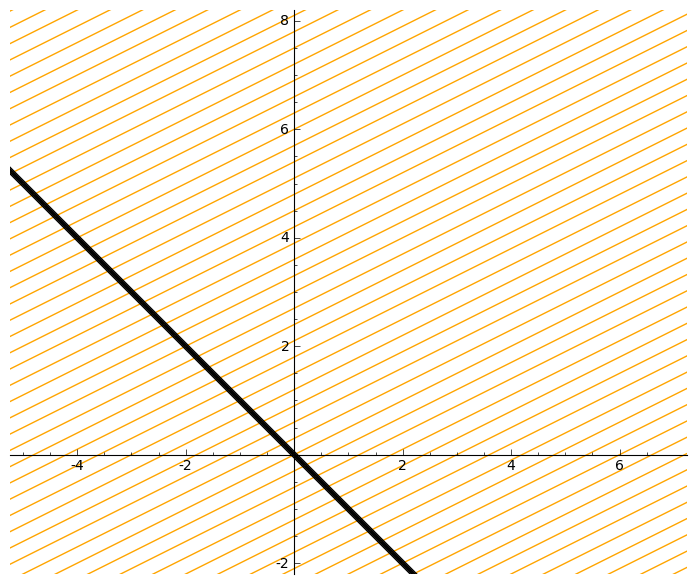
\includegraphics[width=\marginparwidth]{road-corn}}   
\begin{enumerate}
 \item 
What does the vector equation 
$$\pvec{-1\\1}x+\pvec{2\\1}y=\pvec{6\\8}$$ 
have to do with Sally's problem.
 \item 
How would you rephrase the above equation using the language of linear combinations.  Which vector is a linear combination of which vectors?
 \item 
Find values for $x$ and $y$ that make this equation valid.
%\item 
%How far does Sally travel along the road (find the length of $\pvec{-1\\2}x$)?  How far does she travel in the corn?
\end{enumerate}
\end{problem}

The geocaching problem above requires that Sally find out how to obtain the vector $(6,8)$ as a linear combination of the vectors $(-1,1)$ and $(2,1)$.  These two vectors (the road and corn rows) gave us two directions that are independent of each other.  Each direction provides us with a new way to travel that we could not do before. There is only one way to get to the treasure at $(6,8)$ if these are Sally's only two ways to move. Let's examine what happens if we add a third direction, via some irrigation pipes.


\begin{problem}\label{salley in corn field with 3 directions}
 Assume the same conditions as the previous problem. However, now let's assume that in the corn field there are irrigation pipes following the vector $(1,1)$.  Sally now has the option to follow the road $(-1,1)$, the rows of corn $(2,1)$, or the irrigation pipes $(1,1)$. She still wants to get to the treasure at $(6,8)$, but now had 3 options for ways to travel. 
\begin{enumerate}
 \item To get to the treasure, Sally needs to write $(6,8)$ as a linear combination of the vectors $(-1,1)$, $(2,1)$, and $(1,1)$, i.e. she needs to solve
\marginpar{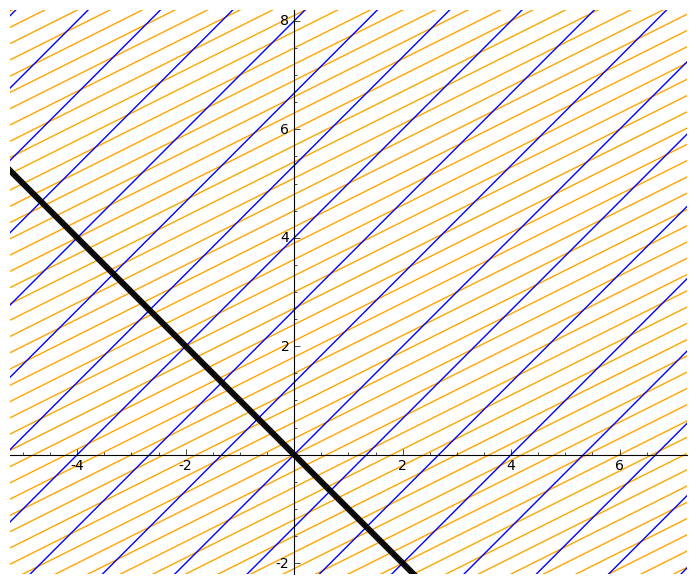
\includegraphics[width=\marginparwidth]{road-corn-pipes}}   
$$\pvec{-1\\1}x+\pvec{2\\1}y+\pvec{1\\1}z=\pvec{6\\8}.$$ 
One such option is $x=3$, $y=4$, and $z=1$.   
Find 3 different ways for Sally to get from the origin $(0,0)$ to the treasure at $(6,8)$. 
 \item Can you find a way to express every possible option that Sally has?
\end{enumerate}
\end{problem}


\mysubsection{\ideagau}

%{\huge This should be up by 4pm today.}
Every time we want to solve a problem involving linear combinations, we can convert that problem into a system of equations.
For example, if we want to write $\pvec{-4\\-15\\9}$ as a linear combination of $\pvec{1\\2\\-1}$, $\pvec{3\\4\\-2}$, and $\pvec{-2\\-10\\6}$, then we would write 
$$ 
\pvec{1\\2\\-1}x_1+\pvec{3\\4\\-2}x_2+\pvec{-2\\-10\\6}x_3=\pvec{-4\\-15\\9}
\quad \text{or}\quad
\bvec{\nvec{1\\2\\-1}&\nvec{3\\4\\-2}&\nvec{-2\\-10\\6}}\bvec{x_1\\x_2\\x_3}=\bvec{-4\\-15\\9},
$$
which as a system of equations becomes
\begin{align*}
x_1+3x_2-2x_3&=-4 \\
2x_1+4x_2-10x_3&=-15 \\
-1x_1-2x_2+6x_3&=9 
\end{align*}

You've solved systems of this form in the past. In this chapter we'll learn an efficient algorithm for solving these systems.

\begin{problem}[Organized Substitution]
Our goal on this problem is to solve the system of equations 
\begin{align*}
x+3y-2z&=-4 \\
2x+4y-10z&=-15\\
-1x-2y+6z&=9. 
\end{align*}
To solve this system, we'll use organized substitution. 
\begin{enumerate}
 \item The first equation is easy to solve for $x$. Solve for $x$ and circle your result. Then replace $x$ with this in both of the other equations. After substituting, you should be able to rewrite each equation in the form $0x+?y+?z=?$.
 \item One of these two simplified equations is easy to solve for $y$.  Solve this equation for $y$ (you shouldn't need fractions), and write your answer in the form $y=?z+?$. Circle this result.  Use this to replace $y$ in the other equation and simplify so you have $0x+0y+?z=?$. 
 \item At this point you should be able to solve for $z$. Circle your result.  Then use this result to find $y$ in your circled equation for $y$.  Then use both values for $z$ and $y$ to obtain $x$ in your circled equation for $x$.   If you ended up with $z=3/2$, then you're on the right track. 
\end{enumerate}
\end{problem}



\begin{problem}[Gaussian Elimination]
We'll now use elimination to solve the system of equations 
\begin{align*}
x+3y-2z&=-4 \\
2x+4y-10z&=-15 \\
-1x-2y+6z&=9. 
\end{align*}
\begin{enumerate}
 \item 
\marginpar{Start by making sure that the coefficient in front of $x$ on the top row is not zero. Swap rows if needed, and then multiply both sides of the top equation by a constant so that you have a 1 in this spot. Then add a multiple of this equation to every other equation to eliminate $x$ from the other equations. }%
The first equation has a 1 as the coefficient in front of $x$. Add a multiple of the first equation to every other equation so that you eliminate the $x$ variable from the other equations.
Write your system in the form 
\begin{align*}
x+3y-2z&=-4 \\
0x+?y+?z&=? \\
0x+?y+?z&=?. 
\end{align*}
 \item One of these two simplified equations is easy to solve for $y$. If you need to swap equations 2 and 3, or multiply both sides of an equation by some constant, do so now so that you can rewrite the system in the form 
\marginpar{If you ignore the top row and the variable $x$, then at this point we just repeat the above process with $y$. Make sure the coefficient in front of $y$ is 1, and then add multiples of the second equation to each lower equation to eliminate $y$.}%
\begin{align*}
x+3y-2z&=-4 \\
0x+1y+?z&=? \\
0x+?y+?z&=?. 
\end{align*}
Then add a multiple of the second equation to the third equation so that you eliminate the $y$. 
Rewrite your system in the form 
\begin{align*}
x+3y-2z&=-4 \\
0x+y+?z&=? \\
0x+0y+?z&=?. 
\end{align*}
\item 
\marginpar{We now ignore the top 2 rows and variables $x$ and $y$, and then repeat the elimination process again. We make sure to get the coefficient in front of $z$ to be a 1. Since there are no more rows beneath this third, we are done. If there had been more rows, we would just keep going.  }%
Multiply the third equation by some nonzero constant so that the coefficient in front of $z$ is a 1. Rewrite the system one final time as
\begin{align*}
x+3y-2z&=-4 \\
0x+y+?z&=? \\
0x+0y+z&=?. 
\end{align*}
 You now have $z$. Use your value for $z$ to quickly obtain $y$ from the second equation, and then $x$ from the first equation.
\end{enumerate}
\end{problem}



\begin{observation}
 
When solving the above system with substitution, we 
\begin{enumerate}
 \item 
picked an equation for which it was easy to solve for a variable, 
 \item
solved for that variable, and then 
\item
replaced that variable in the other equations and simplified each equation. 
\end{enumerate}
We then leave the picked equation alone, and repeat this process on the remaining simplified equations. 

When solving the above system with elimination, we 
\begin{enumerate}
 \item 
picked an equation that we could use to eliminate a variable from the other equations, interchanging this equation with one higher up if needed, 
 \item
multiplied the chosen equation by a nonzero constant to make the leading coefficient 1, and then 
 \item 
added a multiple of the chosen equation to the other equations to eliminate the variable from the other equations. 
\end{enumerate}
We then left the picked equation alone, and repeated this process on the remaining simplified equations below it. 
\end{observation}

These two processes (organized substitution and Gaussian elimination) are fundamentally the same process. You should have noticed that your intermediate steps were the same. We now develop a way to replicate both of these processes with matrices.

\begin{problem}[Gaussian Elimination with Matrices]\
%\marginpar{Follow this link to watch a video of how to perform Gaussian elimination with matrices.}%
Let's solve the same system 
\begin{align*}
x+3y-2z&=-4 \\
2x+4y-10z&=-15 \\
-1x-2y+6z&=9. 
\end{align*}
but now we will only write the coefficients of our system in a matrix. The matrix helps us organize our work, and we have less to write. 
\begin{enumerate}
\item 
\marginpar{This matrix is called the augmented matrix of the system. The vertical bar you see is optional, and is often used to help people remember that there is an equal sign there.} % 
Start by writing the coefficients of system in the matrix (fill in the blanks) 
$$\bvec{[ccc|c]
1 & 3 & -2 & -4 \\
2 & ? & ? & -15 \\
? & ? & 6  & ?}.
$$
\item 
\marginpar{I often write the row operation next to the row I am about to replace. }
Since the upper left entry is a 1, we are ready to reduce.  Add a multiple of row 1 to both row 2 and row 3 (replacing the old row 2 and 3) so that you obtain a zero in both entries below the leading 1 in the top row. Write your work as
$$
\nvec{\bvec{[ccc|c]
1 & 3 & -2 & -4 \\
2 & ? & ? & -15 \\
? & ? & 6  & ?}
\nvec{[l] \\ R_2-2R_1   \\ R_3+?R_1 }
}
\Rightarrow
\nvec{\bvec{[ccc|c]
1 & 3 & -2 & -4 \\
0 & ? & -6 & ? \\
0 & 1 & ?  & ? }
}.
$$
 \item Swap $R_2$ and $R_3$. This should get you a $1$ as the first nonzero entry in row 2. Then you can add a multiple of row 2 to row 3 to obtain a zero below this 1. Write your work in the form 
$$
\nvec{\bvec{[ccc|c]
1 & 3 & -2 & -4 \\
0 & ? & -6 & ? \\
0 & 1 & ?  & ? }
\nvec{[l] \\ R_2\leftrightarrow R_3   \\  }
}
\Rightarrow
\nvec{\bvec{[ccc|c]
1 & 3 & -2 & -4 \\
0 & 1 & ? & ? \\
0 & ? & -6  & ? }
\nvec{[l] \\ \\ R_3+?R_2 }}
\Rightarrow
\nvec{\bvec{[ccc|c]
1 & 3 & -2 & -4 \\
0 & 1 & ? & ? \\
0 & 0 & ?  & 3 }
}
.
$$
 \item Multiply row 3 by some nonzero constant so that the first nonzero entry in row 3 is a 1.  Write your work as
$$
\nvec{\bvec{[ccc|c]
1 & 3 & -2 & -4 \\
0 & 1 & ? & ? \\
0 & 0 & ?  & ? }
\nvec{[l] \\ \\ ?R_3 }}
\Rightarrow
\nvec{\bvec{[ccc|c]
1 & 3 & -2 & -4 \\
0 & 1 & ? & ? \\
0 & 0 & 1  & ? }
}
$$ 
\item Now rewrite your matrix as a system of equations.  The last line row of your matrix, after rewriting it as a system, should be $z=3/2$. Use this to find $y$ and $x$. 
\end{enumerate}
\end{problem}

In our work above, our process was precisely the same as when we used elimination without matrices. When working with equations, we can always (1) interchange the order of equations without changing the solution set to the system.  We can also (2) multiply both sides of an equation  by a nonzero number without affecting the solutions.  Finally, (3) adding a multiple of one equation to another will not affect the solution set. When working with matrices, these three operations on equations become operations on rows of a matrix.  

\begin{definition}[Row Operations]
We define allowed row operations.
\begin{enumerate}
  \item Interchange two rows.
  \item Multiply a row of a matrix by a nonzero constant.
  \item Add a nonzero multiple of a row to another row.
\end{enumerate}
\end{definition}

The row operations above are precisely what we used to row reduce our matrix. The elimination process begins with the first column. We obtain a 1 in the top of that column by (1) swapping rows and/or  (2) multiplying a row by a nonzero scalar. We then (3) add multiples of the first row to the other rows to obtain zeros below this leading 1.  We then ignore the row and column containing this leading 1, and repeat the reduction on the remaining part of the matrix. We can summarize the reduction algorithm with the diagram below.
$$
\bvec{[ccc|c]
* & * & * & * \\
* & * & * & * \\
* & * & * & * \\
}
\Rightarrow
\bvec{[ccc|c]
1 & * & * & * \\
0 & * & * & * \\
0 & * & * & * \\
}
\Rightarrow
\bvec{[ccc|c]
1 & * & * & * \\
0 & 1 & * & * \\
0 & 0 & * & * \\
}
\Rightarrow
\bvec{[ccc|c]
1 & * & * & * \\
0 & 1 & * & * \\
0 & 0 & 1 & * \\
}.
$$
The matrix at the far right provides us with enough information to quickly obtain a solution. After reducing the matrix to this form, we say the matrix is in row echelon form. 

\begin{definition}[Row Echelon Form, Leading 1, Pivot Column]
We say a matrix is in row echelon form (ref) if it satisfies each of the following conditions:
\begin{itemize}
  \item each nonzero row begins with a 1 (called a leading 1),
  \item the leading 1 in each row occurs further right than the leading 1 in the row above, and
  \item any rows of all zeros appear at the bottom.
\end{itemize}
The position in the matrix where the leading 1 occurs is called a pivot.
The column containing a pivot is called a pivot column.
\end{definition}




\begin{problem}[Gauss-Jordan Elimination]
%\marginpar{See YouTube for a video }
Consider the three planes 
$2x+3y+4z=4$, 
$x+2y=6$, and 
$-x+y+2z=0$. 
Let's find the point of intersection by applying row operations to the augmented matrix
$$
A
=
\bvec{
2&3&4&4\\
1&2&0&6\\
-1&1&2&0
}.$$ We'll first obtain row echelon form, and then continue reducing the matrix until we obtain what is called reduced row echelon form. See the link on the right if you would like to watch a video of this reduction process.
\begin{enumerate}
 \item Apply Gaussian elimination to obtain a row echelon form for $A$. You should start by interchanging the first and second rows, so that you have a 1 in the upper left. Remember the pattern 
\marginpar{We say a matrix is in row echelon form when (1) each nonzero row begins with a leading 1, (2) a leading 1 appears to the right of any leading one above it, and (3) any rows of all zeros appear at the bottom.}
$$
\bvec{
2&3&4&4\\
1&2&0&6\\
-1&1&2&0
}
\Rightarrow
\bvec{[ccc|c]
1 & * & * & * \\
0 & * & * & * \\
0 & * & * & * \\
}
\Rightarrow
\bvec{[ccc|c]
1 & * & * & * \\
0 & 1 & * & * \\
0 & 0 & * & * \\
}
\Rightarrow
\bvec{[ccc|c]
1 & * & * & * \\
0 & 1 & * & * \\
0 & 0 & 1 & * \\
}
$$
\item Let's now use row operations (instead of back substitution) to find the solution.  Starting on the right, and working left, use the 1's in each pivot column to reduce the matrix.  Use the pattern 
\marginpar{We say a matrix is in reduced row echelon form when the matrix is in row echelon form, and there are zeros above each pivot. }
$$
\bvec{[ccc|c]
1 & * & * & * \\
0 & 1 & * & * \\
0 & 0 & 1 & * \\
}
\Rightarrow
\bvec{[ccc|c]
1 & * & {\bf 0} & * \\
0 & 1 & {\bf 0} & * \\
0 & 0 & 1 & * \\
}
\Rightarrow
\bvec{[ccc|c]
1 & {\bf 0} & 0 & * \\
0 & 1 & 0 & * \\
0 & 0 & 1 & * \\
}
$$
to complete your reduction. State the point of intersection of the planes.
\marginpar{Check your answer with the technology link \href{http://bmw.byuimath.com/dokuwiki/doku.php?id=visualizing\_systems\_of\_equations}{Visualizing Systems of Equations}.}
\end{enumerate}
\end{problem}


The process above is called Gauss-Jordan elimination. The forward phase of reduction results in a matrix in row echelon form.  We then work backwards starting with the right most pivot column, and use the leading 1 to eliminate the zeros above it.

\begin{definition}[Reduced Row Echelon Form (rref)]
We say that a matrix is in reduced row echelon form (rref) if 
\begin{itemize}
\item the matrix is in row echelon form, and 
\item each pivot column contains all zeros except for the leading 1 in the pivot.
\end{itemize}
\end{definition}

The row reduction process we've described above may not always result in a unique solution. 

\begin{problem}
On this problem, you'll be using software to obtain the rref of a matrix.  The Sage command is ``A.rref()'' and the Mathematica command is ``RowReduce.'' 
\marginpar{You can use the \href{\urlrref}{Sage RREF Calculator} to check your result. Follow the link.}%
\begin{enumerate}
 \item 
Consider the three planes $x+2y-z=3$, $2x-y+4z=0$, and $-x+2z=4$.  
Use software to obtain the reduced row echelon form (rref) for the matrix
$$
\bvec{
1&2&-1&3\\
2&-1&4&0\\
-1&0&2&4
}.
$$  
What does the reduced matrix tell you about how the planes intersect?

When you present in class, you should always write the original matrix, draw an arrow to the rref of the matrix, and write rref above your arrow. This way the class can see what matrix you reduced, and what the rref is. 
 \item
If I wanted to write the vector $(3,0,4)$ as a linear combination of the vectors $(1,2,-1)$, $(2,-1,0)$, and $(-1,4,2)$, then what should I let $c_1$, $c_2$, and $c_3$ equal so that 
$$ c_1(1,2,-1)+c_2(2,-1,0)+c_3(-1,4,2)=(3,0,4),$$ 
which we could rewrite in the easier to use column form
$$ c_1\pvec{1\\2\\-1}+c_2\pvec{2\\-1\\0}+c_3\pvec{-1\\4\\2}=\pvec{3\\0\\4}.$$
[Hint: What does this have to do with the first part?] 
 \item
Now consider the three planes $x+2y-z=3$, $2x-y+4z=0$, and $-5y+6z=-6$.  
Set up an appropriate augmented matrix (make sure you show us the matrix), and use software to verify that the reduced row echelon form is
$$
\bvec{
1 & 0 & \frac{7}{5} & \frac{3}{5} \\
0 & 1 & -\frac{6}{5} & \frac{6}{5} \\
0 & 0 & 0 & 0
}.
$$
Write the three equations represented by this rref (the third equation may seem silly). 
\item Note that the third column does not have a pivot in it. If we added the equation $z=z$ to our work above, then we could solve for $x$, $y$, and $z$ in terms of the variable $z$. 
\marginpar{Because we can choose the third variable to be anything we want, we call it a free variable. }
Write your work in the form 
$$
 \nvec{x\\y\\z}\,\nvec{=\\=\\=}\,\nvec{? \\ ? \\ z}
\quad \quad \text{and}\quad \quad 
 \pvec{x\\y\\z}=\pvec{? \\ ? \\ 1}z+\pvec{?\\?\\0}.
$$
 
\end{enumerate}

\end{problem}

\begin{definition}[Free Variable]
 The variables in a system of equations each correspond to column of the augmented matrix. Some of the columns are pivot columns, and some are not.  The variables corresponding to the nonpivot columns are called free variables.  You can choose these variables to be any number you want, and the write the solution to the system of equations in terms of the free variables. 
\end{definition}

\begin{problem}
\marginpar{Here's an applicable \href{http://www.youtube.com/watch?v=89QO4t1S-cA&feature=share&list=PL7A2089C33C8EFC84}{YouTube video}. }%
Each of the following augmented matrices requires one row operation to be in reduced row echelon form. Perform the single required row operation, and then write the solution to the corresponding system of equations in terms of the free variables.
\begin{multicols}{2}
\begin{enumerate}
	\item 
$
\begin{bmatrix}[ccc|c]
 1 & 0 & 0 & 3 \\
 0 & 0 & 1 & 1 \\
 0 & 1 & 0 & -2
\end{bmatrix}
$ [Remember, you only get one row operation.]
	\item 
$
\begin{bmatrix}[ccc|c]
 1 & 2 & 0 & -4 \\
 0 & 0 & 1 & 3 \\
 -3 & -6 & 0 & 12
\end{bmatrix}
$ [The second column won't have a pivot, so include the equation $x_2=x_2$.]
	\item 
$
\begin{bmatrix}[ccc|c]
 1 & 0 & 2 & 4 \\
 0 & 1 & -3 & 0 \\
 0 & 0 & 0 & 1
\end{bmatrix}
$
	\item 
$
\begin{bmatrix}[ccccc|c]
 0 & 1 & 0 & 7 & 0 & 3 \\
 0 & 0 & 1 & 5 & -3 & -10 \\
 0 & 0 & 0 & 0 & 1 & 2 \\
 0 & 0 & 0 & 0 & 0 & 0
\end{bmatrix}
$ [There are two free variables in this problem.  One of the free variables is $x_1$.]
\end{enumerate}
\end{multicols}
\end{problem}



Throughout the remainder of this chapter, you'll be asked to obtain the rref of many matrices. Always start by using software to obtain the result. 
\marginpar{You can use the \href{\urlrref}{Sage rref calculator} to row reduce a matrix. You can use this on any device that can access a web browser.} 
Even if the problem asks you to compute the rref by hand, please start by using software. This will save you hours of potentially wasted time. 
If you know what the final answer is, you will be able to recognize that you have made a mistake early in the reduction process.

\mysubsection{\ideaind}

Think back on the opening problems of this chapter. Sally starts at the origin $(0,0)$.   
Because Sally can follow the road $(-1,1)$, she has the ability to move away from $(0,0)$. Using the road, she can use linear combinations of $(-1,1)$ to reach any location on the line $y=-x$. 

The rows of corn $(2,1)$ allow Sally to leave the road. 
She can use a linear combination of $(-1,1)$ and $(2,1)$ to arrive at any final destination in the plane that she wants. 
We say these two vectors $(-1,1)$ and $(2,1)$ are linearly independent because they each expand the places Sally can reach. Neither depends on the other. The vectors provide independent directions.
 
Introducing the third direction of travel $(1,1)$ along the irrigation pipes does not change where Sally can travel to, rather this third vector just increases her options for how to get there. Because of this, we say that $(1,1)$ linearly depends on $(-1,1)$ and $(2,1)$. The three vectors $(-1,1)$, $(2,1)$, and $(1,1)$ are dependent.

\begin{problem}
Read the three paragraphs before this problem. Then answer the following.
\begin{enumerate}
 \item If Sally only uses the road and rows of corn, how many linear combinations of $(-1,1)$ and $(2,1)$ are there that will allow Sally to reach the origin? In other words, solve the linear combination equation $$\pvec{-1\\1}x+\pvec{2\\1}y = \pvec{0\\0}$$ by reducing an appropriate matrix. Make sure you show your reduction steps by hand. 
 \item If Sally is also allowed to use the irrigation pipes, how many linear combinations of $(-1,1)$, $(2,1)$, and $(1,1)$ are there that will allow Sally to reach the origin? Obtain the reduced row echelon form of the matrix $\bvec{-1&2&1&0\\1&1&1&0}$ to give your answer.
 \item 
\marginpar{Because this problem has an answer, we say that $(1,1)$ linearly depends on $(-1,1)$ and $(2,1)$.  }%
Write the vector $(1,1)$ as a linear combination of the vectors $(-1,1)$ and $(2,1)$, i.e. solve the equation  $$\pvec{-1\\1}x+\pvec{2\\1}y = \pvec{1\\1}.$$ 
 \item Can you think of a different third vector so that using this vector would expand Sally's final destination points beyond where she can already get to with the road $(-1,1)$ and rows of corn $(2,1)$? Explain.
\note{I am hoping for two different answers her.  I would like someone to say it's impossible.  I would also like someone to suggest a 3D vector.}
\end{enumerate}

\end{problem}



\begin{definition}[Linear Independence]
We say that a set of vectors $\{\vec v_1,\vec v_2, \ldots, \vec v_n\}$ is linearly independent if the only solution to the homogeneous system $$c_1\vec v_{1}+c_2\vec v_{2}+\ldots+c_n\vec v_{n}=\vec 0$$ is the trivial solution $c_1=c_2=\cdots=c_n=0$. 
If the vectors are not independent, then we say that the vectors are linearly dependent. 
% \item In terms of spans, we say vectors are linearly dependent when one of them is in the span of the other vectors. 
%\begin{itemize}
% \item The span of a set of vectors $\{\vec v_1,\vec v_2, \ldots, \vec v_n\}$ is all possible linear combinations of the vectors. In terms of matrices, the span of a set of vectors is all possible vectors $\vec b$ such that $A\vec x=\vec b$ for some vector $\vec x$, where the vectors $\vec v_i$ are placed in the columns of $A$.
% \item The rank of a matrix is the number of pivot columns of the matrix. To find the rank of a matrix, you reduce the matrix using Gaussian elimination until you discover the pivot columns.
%\end{itemize}
\end{definition}
When a collection of vectors is linearly dependent, it is always possible to write one of the vectors as a linear combination of the others. We say the vectors are linearly dependent because one of the vectors depends on (can be obtained as a linear combination of) the other vectors.


\begin{problem*}[9.5 (do this one)]
 Are the vectors $\vec v_1 = (1,3,5)$, $ \vec v_2=(-1,0,1)$, and $\vec v_3=(0,3,1)$ linearly independent?  Solve the system $c_1\vec v_1+c_2\vec v_2+c_3\vec v_3=\vec 0$ to answer this question. If they are dependent, then write one of the vectors as a linear combination of the others.

 Are the vectors $\vec v_1 = (1,2,0)$, $ \vec v_2=(2,0,3)$, and $\vec v_3=(3,-2,6)$ linearly independent?  Solve the system $c_1\vec v_1+c_2\vec v_2+c_3\vec v_3=\vec 0$ to answer this question.  If they are dependent, then write one of the vectors as a linear combination of the others. 

[Hint: Rewrite each of these problems as a system of 3 equations. From that system of equations, write down the corresponding augmented matrix (it will have a column of all zeros at the right).  Then use software to answer each problem.  You do  not need to show your reduction steps, rather show the matrix you reduced, and the rref.]
\end{problem*}

\begin{problem}\label{rocket booster problem}
Imagine you are in a rocket traveling through space.  The rocket has 4 boosters on it.  The boosters provide thrust in a specific direction (vector), with the ability to adjust how strong the push should be in each direction (possibly even moving backwards in that direction - a two sided booster). The 4 boosters allow movement in the directions $(1,1,2)$, $(0,1,3)$, $(2,1,1)$, and $(-2,1,0)$.
\begin{enumerate}
 \item 
\marginpar{Use the \href{http://bmw.byuimath.com/dokuwiki/doku.php?id=rref\_calculator}{Sage RREF Calculator}.}%
Start by row reducing the matrix 
$\begin{bmatrix}
1 & 0 & 2 & -2 \\
1 & 1 & 1 & 1 \\
2 & 3 & 1 & 0
\end{bmatrix}$ to determine which columns are pivot columns. Use technology to get an answer. Then show your row reduction steps by hand. 

The rest of this problem deals with interpreting your rref.  Please give answers with sentences.
 \item If the 4th booster breaks, could some linear combination of the first three rocket thrusts allow you to move in the direction of the 4th rocket? In other words, is it possible to write $(-2,1,0)$ as a linear combination of $(1,1,2)$, $(0,1,3)$, and $(2,1,1)$? Explain.
 \item If the 3rd booster breaks, show that some linear combination of the other three rocket thrusts allows you to move in the direction of the 3rd rocket. What matrix should you row reduce to answer this. Show the class the matrix you started with, and its rref. You do not need to show by hand any reduction steps. Then write $(2,1,1)$ as a linear combination of the other three vectors. 
 \item You have been asked to give advice on a new rocket design. The designers figure that as long as they pick 3 directions in which to provide thrust, they should be able to fly in any direction they want. They attach boosters which allow movement in the directions $(1,3,2)$, $(-3,1,4)$, $(0,1,1)$. Set up an appropriate matrix and use software to row reduce the matrix. What advice would you give the designers?
 \item What does any of the above have to do with linear independence and linear dependence?
\end{enumerate}
\note{In class, I would like to talk about what it would take to design a rocket so that any of the three rockets could go out, and you would still be able to move freely in space.  All they would need is an rref that I followed by a column with no zero entries.  But I would like them to figure this out.  I may just make this a problem later on. 

Follow up.  I did make it a problem later on.}
\end{problem}



 



\begin{problem}
\marginpar{Use the \href{http://bmw.byuimath.com/dokuwiki/doku.php?id=rref\_calculator}{Sage RREF Calculator}.}%
Start by finding the reduced row echelon form of the matrix
$$
B = 
\begin{bmatrix}
\nvec{2\\1}&
\nvec{6\\3}&
\nvec{-1\\1}&
\nvec{2\\5}&
\nvec{0\\1}&
\nvec{1\\0}&
\nvec{3\\3}
\end{bmatrix}.
$$
Show the steps you used to row reduce this matrix. 
The point to this problem is to help you see how this single row reduction can answer all of the questions below. 
\begin{enumerate}
 \item Write $(2,5)$ as a linear combination of $(2, 1)$ and $(-1,1)$. Remember, that when writing $c_1(2,1)+c_2(-1,1)=(1,0)$, you must solve for the unknown constants. Feel free to row reduce the augmented matrix  
$\begin{bmatrix}
\nvec{2\\1}&
\nvec{-1\\1}&
\nvec{2\\5}
\end{bmatrix}
$
with technology. You don't need to show any steps of the computation.
 \item Write $(0,1)$ as a linear combination of $(2, 1)$ and $(-1,1)$. Remember, that when writing $c_1(2,1)+c_2(-1,1)=(0,1)$, you must solve for the unknown constants. If you decide to row reduce the matrix
$\begin{bmatrix}
\nvec{2\\1}&
\nvec{-1\\1}&
\nvec{0\\1}
\end{bmatrix}
$, then use technology and don't show us any of the intermediate steps. 
 \item Continue to write each of $\pvec{1\\0}$, $\pvec{3\\3}$, and $\pvec{6\\3}$ as a linear combination of $\pvec{2\\1}$ and $\pvec{-1\\1}$. [Hint: At some point, rather than row reducing 
$\begin{bmatrix}
\nvec{2\\1}&
\nvec{-1\\1}&
\nvec{a\\b}
\end{bmatrix}
$, ask how you could use the larger matrix to answer this.]
\item The following matrix row reduces to give
$$\begin{bmatrix}
1 & 0 & 2 & 4 & 5 & 8 \\
0 & 2 & -6 & 2 & -1 & 3 \\
0 & -2 & 6 & 0 & 2 & 1
\end{bmatrix}
\xrightarrow{\text{rref}}
\begin{bmatrix}
1 & 0 & 2 & 0 & 3 & 0 \\
0 & 1 & -3 & 0 & -1 & -\frac{1}{2} \\
0 & 0 & 0 & 1 & \frac{1}{2} & 2
\end{bmatrix}
.$$
Write $(5,-1,2)$ as a linear combination of the pivot columns.
\end{enumerate}
 
\end{problem}

\begin{question}
 What connection is there between the rref of a matrix and the columns of the matrix?
\end{question}

\mysubsection{\ideaeig}
\begin{problem}
The following parts ask you to look for points in a vector field where the vector field pushes either straight outwards from the origin, or pulls straight towards the origin.
\begin{enumerate}
\item
Consider the vector field $\vec F(x,y) = \bvec{3&2\\0&2}\bvec{x\\y} = \bvec{3x+2y\\2y}$. 
Compute $\vec F(x,y)$ for each of $(x,y)$ equal to $(2,2)$, $(2,1)$, $(2,0)$, $(2,-1)$, and $(2,-2)$.  Then circle the two vectors $(x,y)$ where the output $F(x,y)$ is a linear combination of the input $(x,y)$. 
For example, if $(x,y)=(-4,2)$, then we compute $\vec F(-4,2) = (-8, 4)$ and we see that $(-8,4) = 2(-4,2)$.  We have $\vec F(x,y) = 2(x,y)$.
 \item Suppose you knew that there was a direction in which the vector field 
$\vec F(x,y) = \bvec{2&5\\4&1}\bvec{x\\y} = \bvec{2x+5y\\4x+y}$ causes a radial push outwards of 6 units. This would mean there exists $(x,y)\neq(0,0)$ such that 
$$\bvec{2&5\\4&1}\bvec{x\\y} = 6\bvec{x\\y}.$$
Find a nonzero vector $(x,y)$ that satisfies this equation.

[Hint: Subtract $6\bvec{x\\y}$ from both sides. Combine terms to get a new matrix to row reduce, and then row reduce the matrix. You should find there are infinitely many correct answers.] 

\end{enumerate}
\end{problem}


\begin{problem}
 Consider the matrix $A=\bvec{1&-1\\3&5}$.
\begin{enumerate}
 \item Explain why solving the problem $A\vec x = c\vec x$ can be done by row reducing the matrix $\bvec{[cc|c]1-c&-1&0\\3&5-c&0}$.
 \item Let $c=3$. Solve $A\vec x = 3\vec x$ by row reducing an appropriate matrix. How many solutions are there?
 \item Let $c=2$. Solve $A\vec x = 2\vec x$ by row reducing an appropriate matrix. How many solutions are there?
 \item  When you row reduce a matrix, what must occur for there to be infinitely many solutions?   
  Can you find another value of $c$ where there are infinitely many solutions to this problem?
\end{enumerate}

\end{problem}




\begin{problem}
Consider the matrix 
$A=\bvec{3&4\\2&1}$.  
This matrix gives us the vector field 
$\vec F(x,y) = A\bvec{x\\y}$. 
We would like to find the directions in which the vector field either pulls a point $(x,y)$ directly towards the origin, 
or pushes the point $(x,y)$ directly away from the origin.
\begin{enumerate}
 \item Explain why we seek a solution to $$ A\bvec{x\\y} = c\bvec{x\\y}$$ where $c$ is some constant. Is $(x,y)=(0,0)$ a solution to this equation.  We call this the trivial solution.
 \item Subtract $c\bvec{x\\y}$ from both sides above.  Show that to find a nonzero $(x,y)$, we need to row reduce the matrix $\bvec{[cc|c]3-c&4&0\\2&1-c&0}$. Then use row operations to eliminate the 2 in the lower left of the matrix. [Hint: Take row 2 and multiply it by $(3-c)$.  Then add $-2$ times row 1 to row 2.]
 \item We already know that $(x,y)=(0,0)$ is a solution.  We want a nonzero solution $(x,y)$. Explain why the bottom row must reduce to be all zeros?
 \item By forcing the bottom row to consist of all zeros, you should have a quadratic equation involving $c$. Solve this equation for $c$.  
 These are the scalars for which you can find a vector that either pushes directly out or pulls directly in. 
\end{enumerate}
\end{problem}

The numbers $c$ that you computed above are called eigenvalues. Note that to find the eigenvalues, we wanted to row reduce a matrix and obtain infinitely many solutions. We'll return to this idea throughout the chapter.  

\mysubsection{\ideamul}

When we solve equations of the form $ax=b$ with numbers, we simply multiply both sides by $\frac{1}{a}$ to obtain $x=\frac{1}{a}b$. This is because for any nonzero number $a$, we have an inverse $a^{-1}$ such that $a^{-1}a = 1=aa^{-1}$. 
 
\begin{definition}[$I_n$ and $A^{-1}$]
 The identity matrix $I$ is a square matrix so that if $A$ is a square matrix, then $IA=AI=A$. The identity matrix acts like the number 1 when performing matrix multiplication. We write 
$$I_2 = \bvec{1&0\\0&1}, 
\quad I_3 = \bvec{1&0&0\\0&1&0\\0&0&1},
\quad I_4 = \bvec{1&0&0&0\\0&1&0&0\\0&0&1&0\\0&0&0&1},
 \text{etc.}$$ 

 If $A$ is a square matrix, then the inverse of $A$ is a matrix $A^{-1}$ where we have $AA^{-1}=A^{-1}A=I$, provided such a matrix exists.
\end{definition}



\begin{problem}
Let 
$A=
\begin{bmatrix}
\nvec{1\\3}&
\nvec{2\\4}
\end{bmatrix}
.$
We now develop an algorithm for computing the inverse $A^{-1}$.
If an inverse matrix exists, then we know it's the same size as $A$, so we could let $A^{-1}=\begin{bmatrix}\vec v_1 & \vec v_2\end{bmatrix}$ be the inverse matrix, where $\vec v_1$ and $\vec v_2$ are the columns of $A^{-1}$.  
\begin{enumerate}
 \item  We know that $A A^{-1} = \begin{bmatrix}\nvec{1\\0}&\nvec{0\\1}\end{bmatrix}.$ 
Explain why $A\vec v_1=\pvec{1\\0}$ and $A\vec v_2=\pvec{0\\1}$.
 \item Solve the matrix equations $A\vec v_1=\pvec{1\\0}$ and $A\vec v_2=\pvec{0\\1}$ by row reducing 
$
\begin{bmatrix}[cc|c]
\nvec{1\\3}&
\nvec{2\\4}&
\nvec{1\\0}
\end{bmatrix}
$
and 
$
\begin{bmatrix}[cc|c]
\nvec{1\\3}&
\nvec{2\\4}&
\nvec{0\\1}
\end{bmatrix}
$.
 \item What is the reduced row echelon form of
$
\begin{bmatrix}[cc|cc]
\nvec{1\\3}&
\nvec{2\\4}&
\nvec{1\\0}&
\nvec{0\\1}
\end{bmatrix}
$? How is this related to your previous work?
 \item State the inverse of $A$. 
\end{enumerate}

\end{problem}

In the previous problem we showed how to obtain a matrix $B$ so that $AB=I$. We now have an algorithm for finding the inverse matrix $A^{-1}$. We augment $A$ by the identity matrix, and then row reduce $[A|I]$ to the matrix $[I|A^{-1}]$.  The inverse shows up instantly after row reduction.


\begin{problem}
 Use the algorithm described immediately before this problem to compute the inverse of 
$$A=\begin{bmatrix}
 3 & 1 & -11 \\
 0 & -1 & 1 \\
 1 & 0 & -4
\end{bmatrix}.$$
Use technology to show you the rref of $[A|I]$, or just use A.inverse() in Sage, or Inverse[A] in Mathematica.  
Then show your row reduction steps by hand.

Once you have obtained the inverse, use your work to write $(1,0,0)$ as a linear combination of the columns of $A$.  
\end{problem}


\mysubsection{\ideaind}


\begin{problem}
For each collection of vectors, use software to determine if the collection of vectors is linearly independent or linearly dependent.  If the vectors are linearly dependent, write one of the vectors as a linear combination of the others. Do not row reduce the matrices by hand, rather on each problem first show the matrix you would row reduce, and then give the reduced row echelon form by using technology.
\begin{enumerate}
 \item $(1,0,0)$, $(0,1,1)$, $(2,3,2)$, and $(0,1,-1)$ 
[Remember, the vectors are linearly independent if the only solution to 
$$\pvec{1\\0\\0}c_1+\pvec{0\\1\\1}c_2+\pvec{2\\3\\2}c_3+\pvec{0\\1\\-1}c_4=\pvec{0\\0\\0}$$ is the trivial solution $c_1=c_2=c_3=c_4=0$.]
 \item $(1,0,2,0)$, $(0,1,3,1)$, and $(0,1,2,-1)$
 \item $(1,1,2,-1)$, $(-3,1,4,1)$, and $(-1,1,3,0)$
 \item Suppose you have 5 vectors that are each 7 tall. Row reducing the 7 by 5 matrix obtained by placing these vectors in columns results in a matrix that has 3 rows of zeros at the bottom.  Why are the vectors linearly dependent?
 \item If you have a matrix with $n$ rows and $m$ columns, what must happen for the column vectors to be linearly independent?  How many rows of zeros would be at the bottom if the vectors are linearly independent. 
\end{enumerate}
[Hint: For all parts, think about the number of pivot columns.]
\end{problem}





\begin{problem}[Rocket Booster Design]
\marginpar{If you are worried about rotation that might occur from firing these boosters, then please imagine that each booster applies a force through the center of mass of the object, so that no rotation occurs.  }%
Three teams have been asked to design a space suit that allows for travel in space. As part of the project requirements, the teams are required to use 4 two-way boosters for propulsion.  The 4th booster is there to allow for redundancy in case any of the the other boosters break. 
\begin{itemize}
 \item Team 1 decides to add boosters to their suit that allows for travel in the directions 
$[1,-1,1],
[1,2,-1],
[3,-1,2],
[1,1,0]$.
 \item Team 2 decides to add boosters to their suit that allows for travel in the directions 
$[1,-3,2],
[0,1,1],
[-1,3,2],
[1,-1,3]$.
 \item Team 3 decides to add boosters to their suit that allows for travel in the directions
$[1,1,-2],
[3,-1,4],
[2,0,1],
[1,-3,8]$.
\end{itemize}
For each team, use software to row reduce the appropriate 3 by 4 matrix that would tell the dependence relationships among the vectors. If you were in charge of picking a winning design, which team would you pick, and why?
\end{problem}


\mysubsection{\ideamul}

\begin{problem}
Start by writing the system of equations 
\begin{align*}
 -2x_1+ 5x_3 &=-2\\
 -x_1+ 3x_3 &=1\\
 4x_1 +x_2  -x_3 &=3
\end{align*} 
as a matrix product $A\vec x =\vec b$.  (What are $A$, $\vec x$ and $\vec b$?)  
\begin{enumerate}
\item 
\marginpar{You should use technology to rapidly compute the inverse and also row reduce the augmented system.  Show by hand any matrix computations you do on  part 3. }%
Use software to find the inverse of the matrix $A$ (state the matrix you row reduced, and the rref of the matrix). 
\item Use software to row reduce the augmented matrix $\begin{bmatrix}[c|c]A&\vec b \ \end{bmatrix}$. State the rref.
\item To solve the problem $ax=b$ where $a$, $x$, and $b$ are numbers, we multiply both sides by $\frac{1}{a}$ to obtain $\frac{1}{a}ax=\frac{1}{a}b$, or because $\frac{1}{a}a=1$, we simplify to get $x=\frac{1}{a}b$. How can you use this idea to solve the matrix problem $A\vec x = \vec b$?  Show how to obtain the solution to this system by using the matrix inverse. 
\item Does it matter if you compute $\vec b A^{-1}$ or  $A^{-1}\vec b$?
%\item What differences do think there are
%$\vec x = \dfrac{1}{A}\vec b$, $\vec x = \dfrac{\vec b}{A}$, and $\vec x = \vec b\dfrac{1}{A}$?   
\end{enumerate}
\end{problem}
\note{At this point I want to talk about order of matrix multiplication.  But it will become much more apparent later on.}



\begin{problem}\label{inverse of 2 by 2}
\marginpar{[Hint: Because the matrix has variables in it, you may want to try a different scheme for row reducing.  Multiply the top row by $c$ and the bottom row by $a$. Then subtract the top row from the bottom. This gets you a zero below the pivot in the first column. Then multiply the top row by $ad-bc$ and the bottom row by something else.]}%
Let $A=\begin{bmatrix}a&b\\c&d\end{bmatrix}$. Obtain the rref of $[A | I]$ to show that the inverse of $A$ is 
$$A^{-1}=\frac{1}{ad-bc}\begin{bmatrix}d&-b\\-c&a\end{bmatrix}.$$

Are there any conditions under which a matrix would not have an inverse?  What are they, and why? Is there a number you could check to {\it determine} if a matrix has an inverse?
\end{problem}

\mysubsection{\ideadet}
In computing the inverse of a 2 by 2 matrix, the number $ad-bc$ appears in the denominator. We call this number the determinant. 
\marginpar{Take a guess as to why we call this number the determinant.  What does it help determine?}% 
If I asked you to compute the inverse of a 3 by 3 matrix, you would again see a number appear in the denominator.  We call that number the determinant. This holds true in all dimensions.

\begin{problem*}[Optional]
  Let $A=\begin{bmatrix}a&b&c\\d&e&f\\g&h&i\end{bmatrix}$. Use Gauss-Jordan elimination to find the inverse of $A$, and show that the common denominator is $a(ei-hf)-b(di-gf)+c(dh-ge)$. 
\end{problem*}


\begin{definition}[Determinants of 2 by 2 and 3 by 3 matrices]\label{determinat of 2 by 2 and 3 by 3}
\marginpar{In Sage, we've been using A.rref() to get the reduced row echelon form of $A$. You can type A.determinant() to get the determinant. Similarly, A.inverse() will get you the inverse. }
 The determinant of a {$2\times 2$} and {$3\times 3$} matrix are the numbers 
\begin{align*}
\det\begin{bmatrix}a&b\\c&d\end{bmatrix} &=\begin{vmatrix}a&b\\c&d\end{vmatrix} = ad-bc\\
\begin{vmatrix}a&b&c\\d&e&f\\g&h&i\end{vmatrix} &= a\det\begin{vmatrix}e&f\\h&i\end{vmatrix} -b\det\begin{vmatrix}d&f\\g&i\end{vmatrix} +c\det\begin{vmatrix}d&e\\g&h\end{vmatrix}\\
&=a(ei-hf)-b(di-gf)+c(dh-ge)
\end{align*}
\marginpar{This approach generalizes to give the determinant of any square matrix.  More on this soon. }% 
We use vertical bars next to a matrix to state we want the determinant. Notice the negative sign on the middle term of the {$3 \times 3$} determinant. 
Also, notice that we can compute three determinants of 2 by 2 matrices in order to find the determinant of a 3 by 3. 
\end{definition}










\begin{problem}
The columns of each matrix below provide the edges of the parallelogram beneath the matrix.
\begin{center}
 \begin{tabular}{ccccc}

$A=\bvec{2&0\\0&3}$
&$B=\bvec{2&1\\0&3}$
&$C=\bvec{1&2\\4&0}$
&$D=\bvec{-2&1\\1&2}$
&$E=\bvec{1&-2\\2&1}$\\\hline
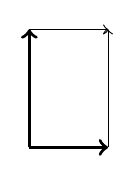
\begin{tikzpicture}[scale=.5] 
\draw[->,very thick] (0,0) -- (2,0); \draw[->,very thick] (0,0) -- (0,3); 
\draw[->] (0,3) -- (2,3); \draw[->] (2,0) -- (2,3); 
\end{tikzpicture}
&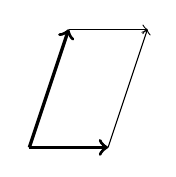
\begin{tikzpicture}[scale=.5] 
\draw[->,very thick] (0,0) -- (2,0); \draw[->,very thick] (0,0) -- (1,3); 
\draw[->] (1,3) -- (3,3); \draw[->] (2,0) -- (3,3); 
\end{tikzpicture}
&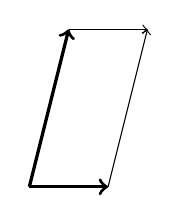
\begin{tikzpicture}[scale=.5] 
\draw[->,very thick] (0,0) -- (1,4); \draw[->,very thick] (0,0) -- (2,0); 
\draw[->] (1,4) -- (3,4); \draw[->] (2,0) -- (3,4); 
\end{tikzpicture}
&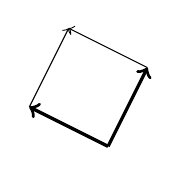
\begin{tikzpicture}[scale=.5] 
\draw[->,very thick] (0,0) -- (-2,1); \draw[->,very thick] (0,0) -- (1,2); 
\draw[->] (-2,1) -- (-1,3); \draw[->] (1,2) -- (-1,3); 
\end{tikzpicture}
&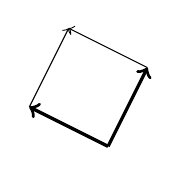
\begin{tikzpicture}[scale=.5] 
\draw[->,very thick] (0,0) -- (-2,1); \draw[->,very thick] (0,0) -- (1,2); 
\draw[->] (-2,1) -- (-1,3); \draw[->] (1,2) -- (-1,3); 
\end{tikzpicture}
\end{tabular}
\end{center}

\begin{enumerate}
\item Compute the determinant of each matrix above. What happens to the determinant when you switch the order of the columns? 
\item Use geometric reasoning to compute the area of each parallelogram ($A=bh$). For the last two, note that the vectors $(-2,1)$ and $(1,2)$ are orthogonal, so the parallelogram is a square. Find the length of each side. 
\item For each parallelogram above, decide if you have to rotate clockwise or counterclockwise to get from the vector in the first column to the vectors in the second column. What does this have to do with the sign of the determinant?
\item Consider the matrix $F=\bvec{ \nvec{3\\2}&\nvec{4\\-1} }$.  Draw the corresponding parallelogram and make a guess as to whether or not the determinant is positive or negative (without computing it). Then compute the determinant and use it to guess the area of the triangle with vertices $(0,0)$, $(3,2)$, and $(4,-1)$.
\end{enumerate}
\end{problem}

The problem above uses inductive reasoning (lots of examples) to suggest that the determinant of a matrix (up to a sign) is the area of a parallelogram. This next problem asks you to use deductive reasoning to prove that the determinant of a 2 by 2 matrix gives the area of a parallelogram whose edges are the columns of the matrix.
\begin{problem}
 To find the area of the parallelogram with vertexes $O=(0,0)$, $P=(a,c)$, $Q=(b,d)$, and $R=(a+b,c+d)$, we need to find the length of $OP$ (the base $b$), and multiply it by the distance from $Q$ to $OP$ (the height $h$). Let $\vec b = \vec{OP}$ and let $\vec h$ be the shortest vector from the line $OP$ to the point $Q$. Complete the following:
\begin{enumerate}
 \item Find the projection of $\vec {OQ}$ onto $\vec {OP}$. (You may need to look up a vector projection formula.) Part of this formula requires that you compute the length of $\vec b$.  
 \item Recall that we can obtain the vector $\vec h$ by computing $\vec h = \vec {OQ}-\text{proj}_{\vec{OP}}\vec{OQ}$. We call this vector is the vector component of $\vec {OQ}$ that is orthogonal to $\vec {OP}$. Compute $\vec h$.
 \item The length of $\vec h$ is the distance $h$ from $Q$ to $OP$. Find the length of $\vec h$.
 \item We now have $b$ and $h$. Compute the product and simplify to show that the area of the parallelogram is $|ad-bc|$.
\end{enumerate}
\end{problem}

The result above extends to 3 dimensions.  The determinant of a 3 by 3 matrix gives the volume of the parallelepiped whose edges are the columns of the 3 by 3 matrix. Because this result holds true in 1, 2, and 3 dimensions, we can use the determinant to define an $n$th dimensional volume. This is precisely what happens in practice. 




\mysubsection{\ideaeig}

There is a connection between linear independence and the determinant.


\begin{problem}
Consider the matrices $A=\bvec{1&-2\\2&-4}$,  $B=\bvec{2&-1\\4&3}$, and $C=\bvec{-2-\lambda&1\\3&4-\lambda}$. (Note that $C = \bvec{-2&1\\3&4}-\lambda \bvec{1&0\\0&1}$.)   
\begin{enumerate}
 \item Compute the determinants of $A$, $B$, and $C$. \marginpar{The determinant of $C$ is called the characteristic polynomial of $\bvec{-2&1\\3&4}$.}
 \item Are the columns of $A$ linearly independent or linearly dependent? Explain.  
 \item Are the columns of $B$ linearly independent or linearly dependent? Explain.
 \item Make a conjecture about determinants and linear independence.  
 \item Find two different values $\lambda$ so that $C$ has linearly dependent columns. (Your answer should involve irrational numbers.)
\end{enumerate}
\end{problem}


A main goal in this chapter has been to answer the following two questions:
\begin{enumerate}
 \item For which nonzero vectors $\vec x$ (eigenvectors) is it possible to write $A\vec x = \lambda \vec x$?
 \item Which scalars $\lambda$ (eigenvalues) satisfy $A\vec x = \lambda \vec x$?
\end{enumerate}
These questions are precisely connected to when a vector causes a radial push away or pull towards the origin. 
Let's give some formal definitions.



\begin{definition}[Eigenvector, Eigenvalue, Characteristic Polynomial]
Let $A$ be a square $n\times n$ matrix. 
\begin{itemize}
 \item An eigenvector of $A$ is a nonzero vector $\vec x$ such that $A\vec x =\lambda \vec x$ for some scalar {$\lambda$}. (Matrix multiplication reduces to scalar multiplication.) We avoid letting $\vec x$ be the zero vector because it is trivially true that $A\vec 0=\lambda \vec 0$ no matter what $\lambda$ is.
 \item If $\vec x$ is an eigenvector with $A\vec x = \lambda \vec x$, then we call $\lambda$ an eigenvalue of $A$.
 \item We call $\det(A-\lambda I)$ the characteristic polynomial of $A$.  It is a polynomial in $\lambda$ of degree $n$, hence has $n$ roots (counting multiplicity).  These roots are the eigenvalues of $A$.
\end{itemize}
\end{definition}




\begin{problem}
 Consider the matrix $A=\bvec{5&6\\3&-2}$. 
\begin{enumerate}
 \item Show that the eigenvalues are $\lambda = 7$ and $\lambda = -4$. You'll want to compute the determinant of $A-\lambda I = \bvec{5-\lambda&6\\3&-2-\lambda}$
 \item If we let $\lambda = 7$, find a nonzero vector $\vec x = (x,y)$ such that $A\vec x = 7\vec x$. You'll need to row reduce $\bvec{[cc|c]5-7&6&0\\3&-2-7&0}$.  
 \item If we let $\lambda = -4$, find a nonzero vector $\vec x = (x,y)$ such that $A\vec x = -4\vec x$.  
 \item If $\lambda = 6$, then what is the only solution $\vec x = (x,y)$ to $A\vec x = 6\vec x$? [Hint: this one can be answered without doing any row reduction.] 
\end{enumerate}

\end{problem}


\begin{problem}
Consider the matrix 
$A=
\begin{bmatrix}
 3 & 1 \\
 4 & 6
\end{bmatrix}
$.
 \begin{enumerate}
 \item Find the characteristic polynomial of $A$, and use it to determine the eigenvalues of $A$. 
 \item For each eigenvalue, find all corresponding eigenvectors. 
% \item Compute the trace and determinant of $A$.
\end{enumerate}
\end{problem}




\begin{problem}
Consider the matrix 
$
A=
\begin{bmatrix}
 6 & 4  \\
 3 & 2  
\end{bmatrix}
$. 
Find the eigenvalues of $A$. 
Then for each eigenvalue, find all corresponding eigenvectors.
%(Check your work by computing the trace and determinant of $A$.)
\end{problem}







\mysubsection{\ideamul}

\begin{problem}[Encryption]
Consider the matrix 
$A =
\begin{bmatrix}
 2&1&-1\\
 5&2&-3\\
 0&2&1
\end{bmatrix}
$.  
Joe decides to send a message to Ben by encrypting the message with the matrix $A$. He first takes his message and converts it to numbers by replacing A with 1, B with 2, C with 3, and so on till replacing Z with 26.  He uses a 0 for spaces.  After replacing the letters with numbers, he breaks the message up into chunks of 3 letters.  He then multiplies each chunk of 3 by the matrix $A$, resulting in a coded message. For example, to send the message ``good job ben'' he firsts converts the letters to the numbers and places them in a large matrix $M$ (top to bottom, left to right) 
$$
\left[\bvec{g\\o\\o}, \bvec{d\\ \ \\ j},\bvec{o\\b\\\  },\bvec{b\\e\\n}\right] 
\rightarrow
\left[\bvec{7\\15\\15}, \bvec{4\\0\\10},\bvec{15\\2\\0},\bvec{2\\5\\14}\right] 
= M=
\begin{bmatrix}
7 & 4 & 15 & 2 \\
15 & 0 & 2 & 5 \\
15 & 10 & 0 & 14  
\end{bmatrix}
.$$
To encode the matrix, he computes 
$$AM = 
\begin{bmatrix}
14 & -2 & 32 & -5 \\
20 & -10 & 79 & -22 \\
45 & 10 & 4 & 24
\end{bmatrix}.$$
and then sends the numbers 
$[
[ 14,  20,  45],
[ -2, -10,  10],
[ 32,  79,   4],
[ -5, -22,  24]]
$ to Ben. Ben uses the inverse of $A$ to decode the message. 
\begin{enumerate}
 \item Find the inverse of $A$. 
 \item Use $A^{-1}$ to decode $[
[ 14,  20,  45],
[ -2, -10,  10],
[ 32,  79,   4],
[ -5, -22,  24]]$ and show the message is ``good job ben''.
 \item Decode the message $[[39, 89, 22],[20, 48,  4],[39, 88, 33]]$.
\end{enumerate}
\end{problem}




\begin{problem}
The eigenvalues of the matrix 
$A=\bvec{2&6\\18&5}$ are $\lambda_1 = 14$ and $\lambda_2 = -7$.  An eigenvector corresponding to $\lambda_1 =14$ is  $\vec x_1=(1,2)$. 
An eigenvector corresponding to $\lambda_2 = -7$ is $\vec x_2 = (-2,3)$. 
\begin{enumerate}
 \item What is the product $A\vec x_1$? What is the product $A\vec x_2$? Can you explain how to get these products without actually doing matrix multiplication.
 \item 
\marginpar{We place the eigenvectors of $A$ into the columns of $Q$.}%
What is the product $AQ$ where $Q = \bvec{\vec x_1&\vec x_2} = \bvec{1&-2\\2&3}$. You can do this product by using your answer to the first part. 
 \item 
\marginpar{[There are several ways to do this problem. You could multiply both sides on the left by the inverse of $Q$ to solve for $D$. Another way is to reason about the connection between eigenvalues, eigenvectors, the matrix $A$, and linear combinations.]
}%
Find a matrix $D$ so that $AQ=QD$.  Any idea why we use $D$ for this matrix? See the hint on the side. 

\item 
Suppose $A$ is a 3 by 3 matrix with eigenvectors $\vec x_1$, $\vec x_2$, and $\vec x_3$, corresponding to the eigenvalues $\lambda = 2,4,-5$, respectively. If we let $Q = \bvec{\vec x_1&\vec x_2&\vec x_3}$, then make a guess as to what $D$ should equal so that $AQ=QD$. Explain your guess. Guess what $D$ equals if we instead place the eigenvectors into $Q$ in the order $Q = \bvec{\vec x_2&\vec x_3&\vec x_1}$? 


\end{enumerate}
%What do they get if they compute AQ (or explain why we immediatly know AQ).  Does it equal DQ or QD.  Does order matter?
%They have to analyze what matrix multiplication means. 
\end{problem}

In the problem above, we wrote $AQ=QD$ where $D$ is a diagonal matrix whose diagonal entries are the eigenvalues of $A$. The columns of $Q$ are eigenvectors of $A$, which we place in the same order as the eigenvalues on the diagonal of $D$. We can use this idea to obtain a matrix with any desired eigenvalue/eigenvector pairs. In particular, this means we can observe something in nature and look for outward/inward pushes/pulls. From these observations we know $Q$ and $D$, which means we can solve for $A$. 


\begin{problem}
Suppose you know that the matrix $A$ has eigenvalues $\lambda_1=2$ and $\lambda_2=-3$ with corresponding eigenvectors $\vec x_1=(2,-5)$ and $\vec x_2 = (1,3)$.
\begin{enumerate}
 \item 
\marginpar{Since $AQ=QD$, what does multiplying both sides by $Q^{-1}$ on the right yield?}%
We can write $AQ=QD$ where $Q=\bvec{\nvec{2\\-1}&\nvec{1\\3}}$ and $D=\bvec{2&0\\0&-3}$. Use this information to solve for $A$.  You can get $Q^{-1}$ quickly from Problem \ref{inverse of 2 by 2}.  Your matrix $A$ should have fractional values in it, with a denominator equal to the determinant of $Q$.
 \item We could have instead written $AQ=QD$ where $Q=\bvec{\nvec{1\\3}&\nvec{2\\-1}}$ and $D=\bvec{-3&0\\0&2}$ (reversing the order we put things into $Q$ and $D$). Use this information to solve for $A$.
 \item Suppose we know that a vector field $\vec F$ applies the forces $F(4,-2) = (8,-4)$ and $F(-1,-3) = (3,9)$. Explain why we know two eigenvectors are $(4,-2)$ and $(3,9)$ with corresponding eigenvalues $\lambda=2$ and $\lambda =-3$.  Use this information to state $Q$ and $D$, and then use $AQ=QD$ to find the matrix $A$ such that $F(x,y)=A\pvec{x\\y}.$
 \item You should have gotten the exact same matrix $A$ in each problem above, though the $Q$ and $D$ used on each part was different. Guess another choice for $Q$ and $D$, different than the three above, so that $AQ=QD$. Why did you make this guess? 
%This problem is most likely best left for a discussion in class.  Let them do the computations. 
% \item We know there are infinitely many eigenvectors corresponding to each eigenvalue of $A$. When we use $AQ=QD$ to find the matrix $A$, does it matter which eigenvectors we choose to put in $Q$?  Does the order we place the eigenvectors in $Q$ make a difference?
\end{enumerate}
\end{problem}

\mysubsection{\ideadet}
Recall that the determinant of a {$2\times 2$} and {$3\times 3$} matrix are the numbers 
\begin{align*}
\det\begin{bmatrix}a&b\\c&d\end{bmatrix} &=\begin{vmatrix}a&b\\c&d\end{vmatrix} = ad-bc\\
\begin{vmatrix}a&b&c\\d&e&f\\g&h&i\end{vmatrix} &= a\det\begin{vmatrix}e&f\\h&i\end{vmatrix} -b\det\begin{vmatrix}d&f\\g&i\end{vmatrix} +c\det\begin{vmatrix}d&e\\g&h\end{vmatrix}\\
&=a(ei-hf)-b(di-gf)+c(dh-ge)
\end{align*}
Notice that we compute three determinants of 2 by 2 matrices in order to find the determinant of a 3 by 3. We now extend this to give a way to compute determinants of any matrix.


\begin{definition}[Minors, Cofactors, and General Determinants]\label{general determinants}
Let {$A$} be an $n$ by $n$ matrix. 
\begin{itemize}
 \item The minor {$M_{ij}$} of a matrix {$A$} is the determinant of the the matrix formed by removing row {$i$} and column {$j$} from {$A$}. 
 \item 
\marginpar{
%\begin{wraptable}[7]{r}{0pt}
%\small
%\begin{tabular}{c}
$\begin{bmatrix}
+&-&+&\cdots\\
-&+&-&\cdots\\
+&-&+&\cdots\\
\vdots&\vdots&\vdots&\ddots
\end{bmatrix}$ 
%\end{tabular}%\end{wraptable}

This sign matrix keeps track of the $(-1)^{i+j}$ portion in the cofactor.
}%
The cofactor $C_{ij}$ is the product of the minor $M_{ij}$ and $(-1)^{i+j}$. This gives $C_{ij} = (-1)^{i+j}M_{ij}$.
 \item To compute the determinant, first pick a row or column.
Then take each entry $a_{ij}$ in that row or column and multiply the entry by its cofactor $C_{ij}$. The determinant is the sum of these products. 

{\bf The determinant is a linear combination of the cofactors of any row or column of the matrix, where we use the entries of that row or column as the scalars.  }

Using summation notation, we can write $|A| = \sum_{k=1}^n a_{ik}C_{ik}$ (if we chose row $i$) or alternatively $|A| = \sum_{k=1}^n a_{kj}C_{kj}$ (if we chose column $j$).  
\end{itemize}
\end{definition}




\begin{problem}
 Compute the determinant of 
$
\begin{bmatrix}
 2 & 3 & -1 \\
 1 & 0 & 0 \\
 4 & 2 & 5
\end{bmatrix}
$
in 3 ways. 
\begin{enumerate}
 \item 
\marginpar{\href{http://www.youtube.com/watch?v=DiULKK1CzR0&feature=share&list=PL7A2089C33C8EFC84}{Watch this relevant YouTube video.}}%
Compute the cofactors of the first row of the matrix, and use them to obtain the determinant. Please show each step of your work, don't just skip straight to an answer. You'll need to explain what you did in class, and you can't do this if you just skip all the steps in between.
 \item Use the cofactors of the second row to obtain the determinant.
 \item Find the determinant by using a linear combination of the cofactors of the third column. 
\end{enumerate}
Note: The determinant, using a linear combination of the cofactors along the second column, is
\begin{align*}
3C_{1,2}+0C_{2,2}+2C_{3,2} 
&= (3)(-1)^{1+2}\begin{vmatrix}1&0\\4&5\end{vmatrix}+(0)(-1)^{2+2}\begin{vmatrix}2&-1\\4&5\end{vmatrix}+(2)(-1)^{3+2}\begin{vmatrix}2&-1\\1&0\end{vmatrix}\\
&= -(3)\begin{vmatrix}1&0\\4&5\end{vmatrix}+(0)\begin{vmatrix}2&-1\\4&5\end{vmatrix}-(2)\begin{vmatrix}2&-1\\1&0\end{vmatrix}\\
&=\cdots \text{(you can finish).}
\end{align*}
\end{problem}




\begin{problem}
 Compute the determinants of the matrices 
$$
A=
\begin{bmatrix}
 2 & 1 & -6 & 8 \\
 0 & 3 & 5 & 4 \\
 0 & 0 & 1 & 5 \\
 0 & 0 & 0 & -4
\end{bmatrix}
\quad\text{ and }\quad
B=
\begin{bmatrix}
 3 & 2 & 5 & -1 \\
 0 & 8 & 4 & 2 \\
 0 & -1 & 0 & 0 \\
 0 & -5 & 3 & -1
\end{bmatrix}
.$$
You can make these problems really fast if you use a linear combination of cofactors where most of the scalars are zero. 
\end{problem}







\begin{problem}

Consider the matrices 
$$
A=
\begin{bmatrix}
1 & 0 & 2  \\
1 & 1 & 1  \\
2 & 3 & 1 
\end{bmatrix}
\quad\quad\text{ and }\quad\quad
B=
\begin{bmatrix}
1 & 0 &  -2 \\
1 & 1 &  1 \\
2 & 3 &  0
\end{bmatrix}.$$
\marginpar{You can use Sage to perform all your work. First store the matrices as A and B. Then use A.inverse(), B.inverse(), A.determinant(), and B.determinant(), etc. to check.}%
These matrices are related to the rocket booster problem (Problem \ref{rocket booster problem}).
\begin{enumerate}
 \item Compute the determinants of $A$ and $B$. Show this part by hand, though you should use software to check your answer. 
 \item Row reduce $A$ and $B$. Use software and just show us the rref.
 \item Are the columns of $A$ linearly independent or linearly dependent? What about the columns of $B$?
 \item Row reduce both $[A|I]$ and $[B|I]$, and then state the inverse of each (or explain why it does not exist).  Use software and just show us the rref.   
 \item How many solutions are there to $A\vec x = \vec 0$?  How many solutions are there to $B\vec x=\vec 0$?
 \item How many solutions does 
$x\pvec{1\\1\\2}+
y\pvec{0\\1\\3}+
z\pvec{2\\1\\1}=
\pvec{0\\0\\0}
$ have?

How many solutions does 
$x\pvec{1\\1\\2}+
y\pvec{0\\1\\3}+
z\pvec{-2\\1\\0}=
\pvec{0\\0\\0}
$ have?
\item Make some conjectures about the relationships you see above. 

\end{enumerate}
\end{problem}


\begin{definition}[Singular]
 We say that a matrix is singular when the determinant of $A$ equals zero, which is precisely when the matrix does not have an inverse. 
\end{definition}






\mysubsection{\ideaeig}

Remember, to find the eigenvalues and eigenvectors of a matrix, we need to find nonzero vector solutions to $(A-\lambda I)\vec x=\vec 0$. This means the determinant of $A-\lambda I$ must be zero, which is the quick formula we use for computing eigenvalues. 

\begin{problem}
Consider the matrix 
$
A=
\begin{bmatrix}
 4 & 0 & 0 \\
 0 & 2 & 1 \\
 0 & 1 & 2
\end{bmatrix}
$. 
Show that the characteristic polynomial of $A$ is $(4-\lambda)(\lambda-3)(\lambda -1)$, and then state the eigenvalues of $A$. 
Then for each eigenvalue, find all corresponding eigenvectors. Show your row reduction steps to get the eigenvectors. (You'll need to row reduce 3 matrices, but with each one the row reduction should be quite fast as the bottom row should reduce to all zeros.)
\end{problem}

\begin{problem}\label{First example of deficient eigenvalue}
Consider the matrices
$
B=
\begin{bmatrix}
 3 & 0 & 0 \\
 0 & 2 & 1 \\
 0 & 1 & 2
\end{bmatrix}
$ and 
$
C=
\begin{bmatrix}
 3 & 1 & 0 \\
 0 & 2 & 1 \\
 0 & 1 & 2
\end{bmatrix}
$.
Feel free to use software on this problem to perform any needed row reductions. 
\begin{enumerate}
\item Show that the characteristic polynomial for both $B$ and $C$ is $(3-\lambda)(\lambda-3)(\lambda -1)$.  What are the eigenvalues?
\item For each eigenvalue of $B$, state all the corresponding eigenvectors. Show us the matrix you need to row reduce, show the rref (from software), and then state the eigenvectors by writing $(x,y,z)$ in terms of the free variables.
\item For each eigenvalue of $C$, repeat the previous step.
\item If you have a repeated eigenvalue, how many linearly independent eigenvectors should you expect to find?
\end{enumerate}
When you are done, you should have written down 4 matrices (2 for each part), each matrix's rref, and then stated the eigenvectors by writing $(x,y,z)$ in terms of the free variables on each part.  
 \end{problem}




\mysubsection{\ideagau}
Recall that there are three types of row operations, namely (1) swap rows, (2) multiply a row by a nonzero constant, and (3) add a multiple of a row to another row.  

When you row reduce the matrix $\bvec{a&b&c\\d&e&f}$ using Gauss-Jordan elimination (or any $2$ by $n$ matrix), we can count the largest number of row operations we'll ever need to perform.  Assume at each stage we decide to swap two rows to get a nice nonzero number in the pivot, and then we multiply that row by a nonzero number to obtain a leading 1. 
With a 2 by $n$ matrix, we would swap rows 1 and 2, and then multiply row 1 by a nonzero number. Then we would add a multiple of row 1 to row 2 to eliminate the entry below this leading 1. We would then multiply row 2 by a nonzero number to obtain a leading 1. Then we'd need one more row operation to eliminate the number above the pivot in column 2. This is a total of 5 operations (we swapped 1 time, multiplied a row 2 times, and added a multiple of a row to another 2 times).  

For larger matrices, how many row operations are needed to perform Gauss-Jordan elimination?
This question is extremely important to computer programming, as the answer related to the time needed for a computer to row reduce a million by million matrix, something that happens all the time since the advent of computers.

%I don't think they will care.....  I'm moving on.
\begin{problem}[Number of operations]
Here's your challenge:  How many row operations are needed to fully reduce an $m$ by $n$ matrix, where $n>m$.
\begin{itemize}
 \item For a 3 by 4 matrix, we would swap rows a maximum of 2 times (once for each row but the last).  We would need to multiply a row by some number 3 times (once for each leading 1). We would add a multiple of a row to another 3 times in the forward elimination and 3 times in the backward elimination (this puts the zeros above and below each pivot). We now have $2+3+6 = 11$ row operations.
 \item Now consider a 4 by 5 matrix. How many row swaps at most will you need?  How many times will you need to multiply to get a leading 1?  How many times will you need to add a multiple of a row to another to get a zero above or below a pivot?  List all these out, then write the number of row operations needed.
 \item Now consider a 5 by 6 matrix. Repeat the above.
 \item Now consider a 6 by 7 matrix. Repeat the above. Did you get $41$ row operations?
 \item Give a formula $f(n)$ so that for each $n$, the number $f(n)$ is the maximum number of row operations. We currently know $f(1)=1$, $f(2)=5$, $f(3)=11$, $f(4)=?$, $f(5)=?$, $f(6)=41$. 
\end{itemize}
If you've never see the online encyclopedia of integer sequences, please head to \href{http://oeis.org/}{http://oeis.org/}. Try the sequence 1, 5, 11, ....  
\end{problem}




\begin{problem}
Let $A=\bvec{6-c&2\\2&3-c}$ where $c$ is a real number.
\begin{enumerate}
 \item For which values of $c$ are the columns of $A$ linearly independent?
 \item For which values of $c$ is the matrix $A$ invertible?
 \item For which values of $c$ are there infinitely many solutions to $A\vec x = \vec 0$?
 \item For which values of $c$ is the determinant of $A$ equal to zero?
 \item For which values of $c$ does the rref of $A$ equal the identity matrix?
 \item For which values of $c$ is the matrix $A$ singular?
 \item For which values of $c$ is $\lambda=0$ an eigenvalue of $A$?
\end{enumerate}
\end{problem}


\mysubsection{\ideaeig}
There are many connections between vector fields and eigenvalues/eigenvectors.  The next three problems have you explore this topic, and make some conjectures.  


\begin{problem}
The following three vector fields are represented by matrices with imaginary eigenvalues. Compute the eigenvalues for each, construct a vector field plot, and on the plot add several trajectories (the path followed by a particle that is dropped into this field). 
\begin{enumerate}
 \item $\vec F(x,y) = \bvec{-1&3\\-2&-4}\bvec{x\\y}=\bvec{-x+3y\\ -2x-4y}=(-x+3y, -2x-4y)$.
 \item $\vec F(x,y) = (x-y, x)$ 
 \item $\vec F(x,y) = (-2y,x)$. 
\end{enumerate}
Make a conjecture as to why one spirals in, one spirals out, and one just wraps around in ellipses. 
\end{problem}




\begin{problem}
Start by downloading the Mathematica notebook \href{https://www.dropbox.com/s/1df1nswgbq3y34n/316-VectorField.nb}{VectorFields.nb (click on the link)}.  The goal of this problem is to make a connection between a vector field and its corresponding eigenvalues/eigenvectors. Once the notebook is open, click somewhere in the text. Hold down Shift and press Enter to evaluate the commands and produce a vector field plot. The eigenvector directions are drawn in green. You can click on the bubbles with crosshairs to adjust the vector field (the adjustable vectors are are the columns of the matrix). Play around with the animation until you feel like you can answer each of the following questions. Write your answers to the first 4 by writing complete sentences, and provide a rough hand sketch of a vector field for each case to match your sentences. 
 \begin{enumerate}
  \item If the vector field pushes things outwards in all directions, what do you know about the eigenvalues?
  \item If the vector field pulls things inwards in all directions, what do you know about the eigenvalues?
  \item How can you tell, by looking at a vector field plot, that one eigenvalue is positive and the other is negative?
  \item If the vector field involves swirling motion, what do you know about the eigenvalues? What makes the difference between spiraling inwards, outwards, or just spinning in circles?
  \item (Challenge) What happens when you have a repeated eigenvalue? This one has lots of correct answers, and it is a topic for much further discussion. See if you can get an example of a repeated eigenvalue with a behavior that's different from the above. 
 \end{enumerate}
If you have the first 4, you can present in class. We'll have you come up to the computer and show us what you did.
\end{problem}



We've already seen how to visualize the solution to a first order systems of ODEs.  All we have to do is draw the corresponding vector field.  The solutions to the ODE are the trajectories that follow the vectors in the field.  In the previous chapter we visualized solutions by drawing a vector field. The next problem has you construct visual graphical solutions by only considering the eigenvalues and corresponding eigenvectors.  The vector field plot is not needed. 

\begin{problem}
Consider the system of ODEs $x'=y$, $y'=8x-2y$. This is a system of ODEs whose solution would give the position $(x,y)$ of a particle whose tangent vectors are $(x',y') = (y, 8x-2y)$.  In other words, solving this ODE will tell us the trajectories we can see from a plot of the vector field  $\vec F(x,y)=(y, 8x-2y)$. 
\marginpar{Once you have finished, you should look at a vector field plot of $\vec F(x,y)=(y, 8x-2y)$. Your trajectory plots should follow the vectors in the vector field plot, but you didn't ever have to make the vector field plot.
}%
On this problem, do not draw the vector field, as the goal is to answer all the questions below by just knowing the eigenvalues and eigenvectors.  
\begin{enumerate}
 \item Write this system of ODEs in the form 
$$\bvec{x'\\y'}=A\bvec{x\\y}=\bvec{\rule{.5cm}{.5pt}&\rule{.5cm}{.5pt}\\ \rule{.5cm}{.5pt}&\rule{.5cm}{.5pt}}\bvec{x\\y}.$$  
 Find the eigenvalues of $A$, and then give an eigenvector for each eigenvalue.
 \item The eigenvectors determine two lines through the origin.  Draw these lines on the same plot. This will divide the plane into 4 parts.
 \item If an object starts at $(2,4)$, draw the path the object will follow. Draw your path in the same plot that contains the lines determined from your eigenvectors. Then repeat this part for each initial condition $(0,4)$, $(-2,4)$, $(-1,4)$, and $(2,-2)$. 
\end{enumerate}
You should have single plot that contains 2 lines, and then 5 trajectories. Two of your trajectories will match up with your lines, but it's important that you note which trajectory moves radially outwards, and which moves radially inwards.
\end{problem}




\section*{Wrap up}
\addcontentsline{toc}{section}{Wrap Up}

This concludes the chapter.  Look at the objectives at the beginning of the chapter. Can you now do all the things you were promised? 


\begin{problem}[Lesson Plan Creation] \marginpar{This counts as 4 prep problems. My hope is that you spend at least an hour creating your one-page lesson plan.}
Your assignment: organize what you've learned into a small collection of examples that illustrates the key concepts. I'll call this your one-page lesson plan. You may use both sides. The objectives at the beginning of the chapter give you a list of the key concepts. Once you finish your lesson plan, scan it into a PDF document (use any scanner on campus), and then upload the document to I-Learn.
\end{problem}




\note{
















%Do this in class in groups.  Don't do it out of class.  This is a QUICK in class group problem. 
\begin{problem}
Consider the matrix 
$
A=
\begin{bmatrix}
 1 & 2 & 1 & 0 \\
 0 & 2 & 1 & 1 \\
 0 & 0 & 2 & 0 \\
 0 & 0 & 0 & 5
\end{bmatrix}
$. 
Find the characteristic polynomial and eigenvalues of $A$. 
Then for each eigenvalue, find all corresponding eigenvectors.
(Check your work by computing the trace and determinant of $A$.)
\end{problem}





%This is begin moved to the next chapter, right around the Cramer's rule part.  It's a great conjecture problem. 
\begin{problem}
 Consider the matrix
$A=\begin{bmatrix}
2&1&-1\\1&2&0\\0&4&3 
\end{bmatrix}.$
 Compute the determinant of $A$.  Then create a matrix $B$ so that the $ij$th entry of $B$ is the cofactor $C_{ij}$ (remove row $i$ and column $j$, compute the determinant, and then times by an appropriate sign).  This will require that you compute nine 2 by 2 determinants.  Finally, compute the inverse of $A$ (feel free to use a computer on this part). Make a conjecture about the connection between the determinant of $A$, this matrix $B$, and the inverse of $A$.  We'll verify your conjecture is true on a 4 by 4 matrix in class. 
\end{problem}


%Define Span... Should this wait.   Yes.!!  Wait till chapter 4.  I'll define vector spaces as spans. Hold off on this one. 
\begin{problem}
 Is the vector $[2, 0, 1, -5]$ in the span of $$\{[1, 0, -1, -2], [1, 2, 3, 0], [0, 1, -1, 2]\}?$$ If it is, then write it as a linear combination of the others.  If it is not, then explain why it is not.
\end{problem}
%The rocket booster problem has already helped them develop the notion of span.  I can use the rocket booster problem to define span and define vector space. 



%I'm not sure this is needed any more.  I've already hit linear combinations to death.  Perhaps they've done enough of this already. 
\begin{problem}
Do each of the following:
\begin{enumerate}
 \item Solve the system of equations $x+2y=3$, $4x+5y=6$.
 \item Write the vector $\pvec{3\\6}$ as a linear combination of $\pvec{1\\4}$ and $\pvec{2\\5}$.
 \item Let $A = \pvec{1&2\\4&5}$ and $\vec b=\pvec{3\\6}$.  Find a vector $\vec x$ so that $A\vec x = \vec b$. This matrix $A$ is called the coefficient matrix of the system in the first part.  
\end{enumerate}
How are these three questions related?
 
\end{problem}



A linear combination of vectors is simply a sum of scalar multiples of the vectors. 
We start with some vectors, stretch each one by some scalar, and then sum the result. 
Much of what we will do this semester (and in many courses to come) relates directly to understanding linear combinations.  

%This is aproblem best left in chapter 1.
\begin{problem}
 The force acting on an object is $\vec F = (-3,2)$ N. The object is in motion and has velocity vector $\vec v=(1,1)$ and acceleration vector $\vec a = (-1,2)$.  Write the force as a linear combination of the velocity and acceleration vectors. 
\end{problem}

%This was put in chapter 1, I believe....
\begin{problem}
 Write the vector $(2,3,1)$ as a linear combination of the standard basis vectors in $\mathbb{R}^3$.  Then write $(2,3,1)$ as a linear combination of the vectors $(1,0,0)$, $(1,1,0)$, and $(1,1,1)$.  
\end{problem}


%Note.  This problem goes great if you first swap rows 1 and 2, and then subtract row 2 from row 2.  The numbers stay small. 
\begin{problem}
 Solve the system of equations 
\begin{align*}
  2x+3y-4z&=4\\  
  3x+4y-3z&=8\\  
  7x+12y-12z&=19.  
\end{align*}
Find the reduced row echelon form.  
\end{problem}

%extra... use if you need more fodder. 
\begin{problem}
Use Gaussian elimination to solve 
 $$
\begin{array}{rl}
  x_2 -2x_3 &= -5 \\
 2x_1 -x_2 + 3x_3 &= 4 \\
 4x_1 +x_2 + 4x_3 &= 5
\end{array}
$$
by row reducing the matrix to reduced row echelon form.
[Hint: Start by interchanging row 1 and row 2.] 
\end{problem}

%extra... use if you need more fodder
\begin{problem}
Use Gaussian elimination to solve 
 $$
\begin{array}{rl}
 x_1 -2x_2 +x_3 &= 4 \\
 -x_1 + 2x_2 + 3x_3 &= 8 \\
 2x_1  -4x_2 +x_3 &= 5
\end{array}
$$
by row reducing the matrix to reduced row echelon form.
[Hint: You should end up with infinitely many solutions. State your solution by writing each variable in terms of the free variable(s).]
\end{problem}

%Great is you need more fodder.
\begin{problem}
Use Gaussian elimination to solve 
 $$
\begin{array}{rl}
 x_1 + 2x_3 + 3x_4 &= -7 \\
 2x_1 +x_2 + 4x_4 &= -7 \\
 -x_1 + 2x_2 + 3x_3  &= 0 \\
 x_2  -2x_3  -x_4 &= 4
\end{array}
$$
by row reducing the matrix to reduced row echelon form.
\end{problem}



%Not needed.  They already did this in the context of a vector field - and that's where the intuition is built.   Could be a great in class problem...  It also emphasizes matrix multiplication, but I would move it to chapter 1.  Actually, that's where this should go. 
\begin{problem}\label{use definition of eigenvectors}
Use the definition above to determine which of the following are eigenvectors of
$
\begin{bmatrix}
 3 & 1 \\
 4 & 6
\end{bmatrix}
$
:
$$\pvec{1\\1}, \pvec{1,4}, \pvec{4\\1}, \pvec{1,\\-1}, \pvec{-2,\\2}.$$   
If the vector is an eigenvector, state the corresponding eigenvalue.
\end{problem}



}
